\chapter{Regularizacija in izbor značilk}

V prejšnjem poglavju smo uporabili računske grafe in gradientni sestop za implementacijo linearne regresije in zaključili pri razlagi. To je, skušali smo interpretirati model s stališča uteži, ki jih je ta dodeli posameznim atributom. Na primeru podatkov s področja zdravstva smo na primer ugotovili, da ima pričakovano najpomembnejši atribut dejansko najvišjo utež, a da hkrati model tudi kombinira vrsto drugih atributov tako, da ustrezno popravi model. Pri tem so nas vsekakor ``zmotile'' tudi visoke korelacije med atributi in pa morda to, da so pri utežeh upoštevani prav vsi atributi iz učne množice. To je, prav vsi atributi so imeli neničelne uteži oziroma smo za uporabo modela morali upoštevati vse atribute. Fino bi recimo bilo, če bi model vseboval samo nekatere atribute in bi ostali imeli utež nič ter bili na ta način izločeni iz modela. Tak model bi bil enostavnejši za uporabo (vanj bi ob uporabi lahko vnesli manj podatkov), morda razumljivši, vsekakor pa bi tudi informacija o tem, katerih atributov ne upošteva, bila lahko koristna.

\begin{margintable}
\begin{tabular}{S S}
\toprule
{$x$} & {$y$} \\
\midrule
0.19 & 0.28 \\
0.09 & 0.24 \\
0.16 & 0.48 \\
0.34 & 0.60 \\
0.59 & 0.71 \\
0.87 & 0.51 \\
0.89 & 0.37 \\
0.68 & 0.62 \\
0.36 & 0.51 \\
0.82 & 0.48 \\
\bottomrule
\end{tabular}
\vspace*{3mm}
\caption{Učni podatki.}
\label{t:poly}
\end{margintable}

Zgornjo idejo izločitve določenih vhodnih spremenljivk iz modela lahko implementiramo s pomočjo postopka, ki se imenuje {\em regularizacija}. A preden jo vpeljemo, začnimo s primerom, kjer lahko dodatni atributi močno škodijo učenju.

\section{Polinomska regresija}

Začnemo s podatki v tabeli~\ref{t:poly}. Ti podatki niso prav nič posebnega, razen po navidezni neprimernosti za linearno regresijo, kar kaže tudi spodnja slika.

\begin{figure}
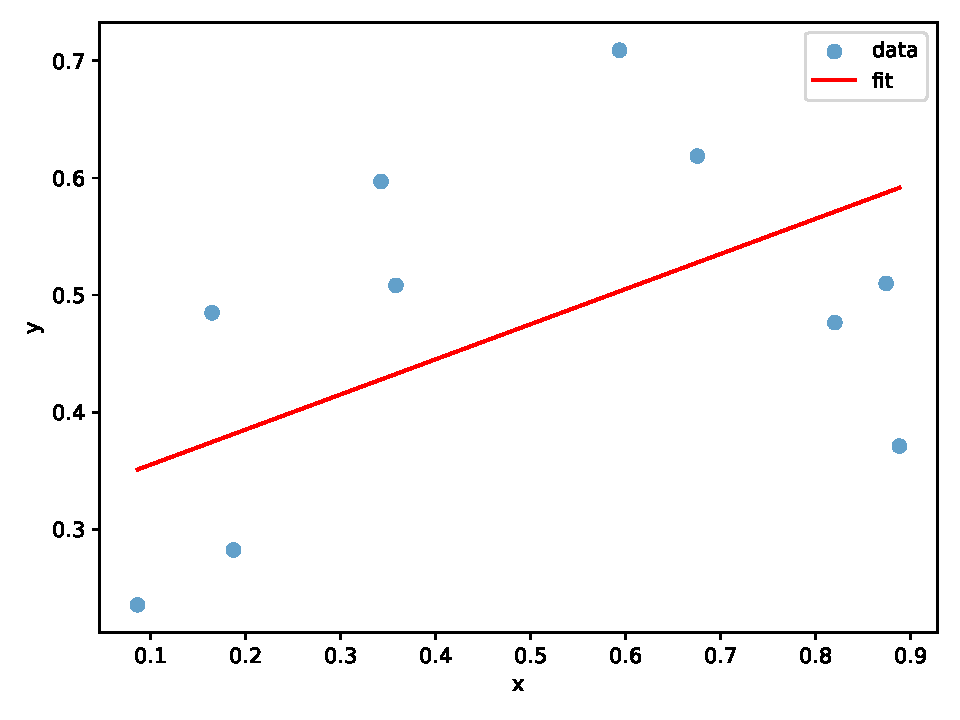
\includegraphics[width=.6\linewidth]{figs/040-lin-plot.pdf}
\caption{Linearna regresija naših začetnih podatkov iz tabele~\ref{t:poly} ne modelira najbolje.}
\end{figure}

Rekli bi lahko, da se te podatke ne da modelirati z linearno regresijo. Ali pač? V tabelo dodajmo nov, izvedeni atribut $x^2$ in naj bo tako dopolnjena tabela vhod za linearno regresijo. Ta bo poiskala uteži atributov za model
%
\begin{margintable}
\begin{tabular}{S S S}
\toprule
{x} & {$x^2$} & {y} \\
\midrule
0.19 & 0.04 & 0.28 \\
0.09 & 0.01 & 0.24 \\
0.16 & 0.03 & 0.48 \\
0.34 & 0.12 & 0.60 \\
0.59 & 0.35 & 0.71 \\
0.87 & 0.76 & 0.51 \\
0.89 & 0.79 & 0.37 \\
0.68 & 0.46 & 0.62 \\
0.36 & 0.13 & 0.51 \\
0.82 & 0.67 & 0.48 \\
\bottomrule
\end{tabular}
\vspace*{3mm}
\caption{Prejšnji tabeli podatkov (tabela~\ref{t:poly}) smo dodali novo kolono oziroma nov atribut, ki smo ga izračunali iz kolone $x$.}
\end{margintable}

\[
y = w_0 + w_1 x + w_2 x^2 .
\]

S tem smo v modelu linearne regresije dodali dodatni atribut. Po obliki naš model sicer ni več linearen v spremenljivki $x$, temveč je kvadraten polinom. Pomembno pa je, da je model še vedno linearen v parametrih ($w_0$, $w_1$, $w_2$), zato lahko zanj uporabimo povsem enak postopek učenja kot prej, torej linearno regresijo. 

Rezultate učenja takega modela lahko znova upodobimo v ravnini $(x,y)$, kot to kaže spodnji graf. Odlično! Model se sedaj dobro prilega učnim podatkom. 
%
\begin{figure}
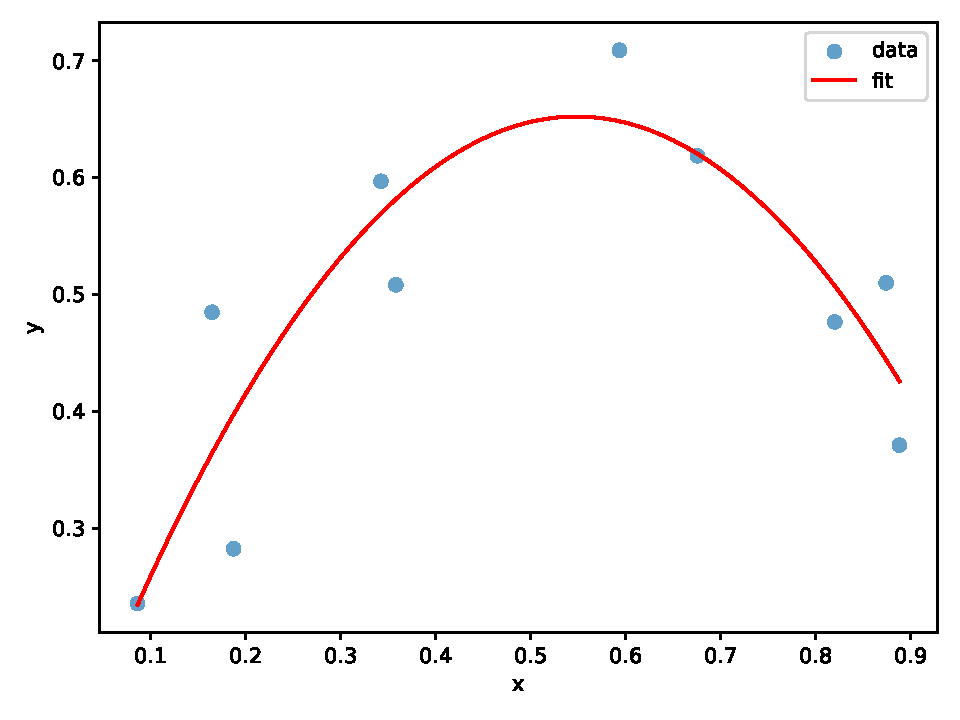
\includegraphics[width=.6\linewidth]{figs/040-poly-plot.pdf}
\caption{Tudi ta model je linearna regresija.}
\end{figure}
%
Tudi vrednost cenovne funkcije, ki jo v linearni regresiji minimiziramo (povprečna vsota kvadratov napak), je veliko manjša kot v primeru, ko v tabelo nismo dodali nove spremenljivke. In sicer se je iz $0.018$ za osnovne podatke zmanjšala na zgolj $0.005$.


Nihče nas sicer ne ovira\marginnote{Tovrstno razširitev učne množice imenujemo {\em polinomska razširitev}, trik, ko to združimo z linearno regresijo pa {\em polinomska regresija}}, da z dodajanjem atributov ne nadaljujemo. Lahko bi namreč dodali še potence višjega reda. Recimo $x^3$, $x^4$, vse do recimo $x^7$. Cenovno funkcijo smo uspeli še malo zmanjšati, tokrat na $0.003$. Uspešno, torej!? 

\begin{figure}
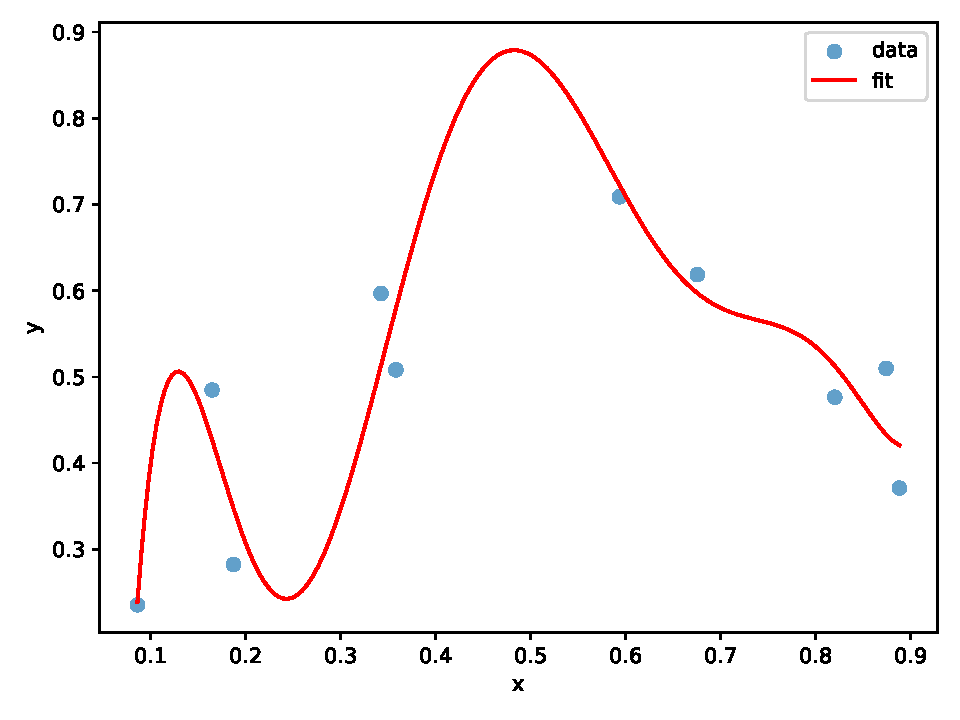
\includegraphics[width=.6\linewidth]{figs/040-poly-plot-7.pdf}
\caption{In tudi to je linearna regresija.}
\end{figure}

Želja po zmanjšanju cenovne funkcije\marginnote{Kaj bi se zgodilo pri dodajanju atributov do polinoma devete stopnje, torej do točke, ko bi vključili tudi $x^9$. Koliko bi bila vrednost kriterijske funkcije takrat? Zakaj?} nas je privedla (skoraj) do ekstrema. Model se je pričel popolnoma prilagajati učni množici in kot tak za napovedovanje ni več uporaben.

\section{Regularizacija L2}

Če si pri zgornjem primeru nekoliko podrobneje ogledamo uteži modela, opazimo zanimiv pojav. Pri modelu druge stopnje so uteži še razmeroma majhne. Ko pa začnemo dodajati nove atribute, torej potence $x^3$, $x^4$, $x^5$ in tako naprej, uteži hitro postanejo zelo velike. Nekatere so pozitivne, druge negativne, njihove absolutne vrednosti pa lahko postanejo tudi več tisočkrat, tudi desettisočkrat večje od vrednosti vhodnih spremenljivk.

To tudi pojasni, zakaj postaja funkcija $y(x)$ oziroma njena odvisnost od vhodne spremenljivke $x$ čedalje bolj zapletena. Velike uteži pomenijo, da lahko že zelo majhna sprememba vhodne spremenljivke $x$ povzroči veliko spremembo v napovedani vrednosti $y$. Model zato začne slediti vsaki malenkostni spremembi v učnih podatkih in s tem pravzaprav modelira tudi šum. Dobljeni model tako sicer zelo dobro prilega učni množici, a postaja za napovedovanje novih primerov neuporaben.

Opazovanje vrednosti uteži pri dodajanju atributov, kot smo jo opazili zgoraj, nas vodi k naslednji ideji. Poleg želje k dobremu prileganju učnim podatkom si pri gradnji linearnega modela lahko zaželimo tudi, da so uteži modela čim manjše ter da je model na ta način enostavnejši. V cenovno funkcijo moramo zato poleg napake modela vključiti še kazen za velike uteži. Ker nas pri tem ne zanima, ali je utež pozitivna ali negativna, uteži kvadriramo. Pri tem običajno izpustimo utež $w_0$, saj ta predstavlja zgolj začetno vrednost funkcije. Cenovna funkcija linearne regresije tako postane
%
\[
J(\mathbf{w}) =
\frac{1}{n} \sum_{i=1}^{n} (y_i - \hat{y}_i)^2
+
\lambda \sum_{j=1}^{p} w_j^2 .
\]

Prvi člen cenovne funkcije je enak temu, ki ga že poznamo, torej povprečni kvadrirani napaki napovedi. Drugi člen pa kaznuje  velike uteži. Ker gre za vsoto dveh členov, ki nista v enakih merskih enotah in tudi konceptualno različna, moramo drugi, novi člen ustrezno utežiti. To storimo s parametrom $\lambda$, ki mu pravimo \emph{stopnja regularizacije}. V implementaciji za regularizacijo torej spremenimo samo izračun funkcije izgube znotraj razreda \texttt{LinReg}, ki implementira linearno regresijo:

\vspace*{3mm}
\begin{lstlisting}
def loss(self, xs, ys):
    yhats = [self(x) for x in xs]
	loss = sum([(y - yhat)**2  for y, yhat in zip(ys, yhats)]) \
	       / Value(len(xs))
    loss += self.reg_strength * sum([w**2 for w in self.weights]) \
            / len(self.weights)
    return loss
\end{lstlisting}
%
Funkcija \texttt{loss} predpostavlja, da smo v razredu primerno inicializirali spremenljivko \texttt{self.reg\_strength}. Regularizacijski člen smo dodatno tudi delili s številom uteži modela, kjer se spomnimo, da sem ni vključenega člena \texttt{self.b}.

Pri stopnji regularizacije $\lambda = 0$ (to je, ko je \texttt{self.reg\_strength} enak 0.0) dobimo natanko isti model kot pri navadni linearni regresiji. Ko vrednost $\lambda$ povečujemo, začne kazen za velike uteži postajati vedno pomembnejša. Model zato raje izbira manjše uteži, posledično pa postaja funkcija $y(x)$ bolj gladka in enostavnejša. Kaj pa se zgodi, če stopnjo regularizacije povečamo na zelo veliko vrednost? V tem primeru drugi člen v cenovni funkciji prevlada in model teži k temu, da so vse uteži čim bližje nič. 

Kolikšna bo v tem primeru vrednost $w_0$? Cenovno funkcijo lahko takrat zapišemo kot
%
\[
J(w_0) = \frac{1}{n} \sum_{i=1}^{n} (y_i - w_0)^2 .
\]
%
Poiščimo minimum te funkcije. Odvajamo po $w_0$:
%
\[
\frac{\partial J}{\partial w_0}
=
\frac{1}{n} \sum_{i=1}^{n} 2(w_0 - y_i).
\]
%
Pri minimumu mora biti odvod enak nič:
%
\[
\sum_{i=1}^{n} (w_0 - y_i) = 0 .
\]
%
Od tod sledi
%
\[
n w_0 = \sum_{i=1}^{n} y_i ,
\]
%
oziroma
%
\[
w_0 = \frac{1}{n} \sum_{i=1}^{n} y_i .
\]

Vidimo torej, da bo model pri zelo veliki stopnji regularizacije napovedoval kar povprečno vrednost učnih podatkov $y$. Kar je silno zanimivo: popolnoma zglajeni model, oziroma najbolje enostaven model, je torej napoved s povprečno vrednostjo.

Postopek\marginnote{Ime izhaja iz oblike optimizacijskega problema: dodatek ($\lambda \sum_j w_j^2$) spremeni površino cenovne funkcije tako, da ima izrazit greben (angl. {\em ridge}) vzdolž smeri, kjer so parametri slabo določeni zaradi močne korelacije med atributi. Regularizacijski člen ta ``greben'' zaobli, zato ima problem enolično rešitev in uteži ostanejo omejene.}, ki smo ga pravkar opisali, imenujemo \emph{regularizacija}. Ker pri tem kvadriramo uteži, govorimo natančneje o \emph{L2 regularizaciji}. Ta pristop je v literaturi pogosto znan tudi kot grebenska regresija (angl. \emph{ridge regression}).

\section{Ocenjevanje točnosti modela z $R^2$}

Pomudimo se še malo pri napovedovanju s povprečno vrednostjo na učni množici. Oziroma, pri najenostavnejšem regresijskem modelu, ki ga torej zgradimo brez upoštevanja vrednosti atributov. Pričakujemo, da bodo modeli, ki bodo upoštevali te vrednosti bolj točni, oziroma da bo njihova napaka manjša. Smiselno bi zato bilo oceniti razmerje med napako, ki jo dobimo pri atributno informiranem modelu in našim osnovnim modelom, kjer napovedujemo s povprečno vrednostjo:

\[
\frac{\sum_{i=1}^{n}(y_i - \hat{y}_i)^2}
{\sum_{i=1}^{n}(y_i - \bar{y})^2},
\]

kjer je $\hat{y}_i$ napoved našega modela, $\bar{y} = \frac{1}{n}\sum_{i=1}^{n} y_i$ pa povprečna vrednost ciljne spremenljivke. Če je vrednost tega količnika blizu $0$, pomeni, da je naš model bistveno boljši od napovedovanja s povprečjem. Če je enaka $1$, je model enako dober kot osnovni model, če pa je večja od $1$, je celo slabši.

Ker si želimo mero, pri kateri večje vrednosti pomenijo boljši model (najbolje blizu $1$) in slabše vrednosti bližje $0$, ta količnik odštejemo od $1$ in dobimo mero $R^2$:

\[
R^2 = 1 - \frac{\sum_{i=1}^{n}(y_i - \hat{y}_i)^2}
{\sum_{i=1}^{n}(y_i - \bar{y})^2}.
\]

Mera $R^2$ je pogosto bolj primerna od mer, kot je RMSE, ker je brezrazsežna in vedno v enakem razponu, torej med 0 in 1\marginpar{Pa je to res? Je možno, da bi kakšen model napovedoval slabše od najenostavnejšega modela? Bo to tako na učni množici primerov ali na novih primerih?}, ter zato omogoča primerjavo točnosti med različnimi podatkovnimi množicami ali problemi. Medtem ko RMSE podaja napako v enotah ciljne spremenljivke, $R^2$ izraža, kolikšen delež variance podatkov pojasni model, kar je pogosto bolj intuitivno. Poleg tega $R^2$ neposredno primerja model z osnovnim pristopom napovedovanja s povprečjem, zato takoj pove, ali model dejansko prinaša izboljšavo.

\section{Regularizacija L1}

Pri L2 regularizaciji smo kaznovali velike uteži tako, da smo v cenovno funkcijo dodali vsoto njihovih kvadratov. Uteži so se zato sicer zmanjšale, vendar praviloma nobena od njih ni postala natanko enaka nič. Model je tako še vedno uporabljal vse atribute, le z nekoliko manjšimi utežmi. Če pa je naš cilj, da bi model nekatere atribute povsem izločil, potrebujemo nekoliko drugačen pristop. Namesto kvadratov uteži lahko v cenovno funkcijo vključimo vsoto njihovih absolutnih vrednosti. Dobimo cenovno funkcijo

\[
J(\mathbf{w}) =
\frac{1}{n} \sum_{i=1}^{n} (y_i - \hat{y}_i)^2
+
\lambda \sum_{j=1}^{p} |w_j|.
\]

Kaj se zgodi, ko povečujemo stopnjo regularizacije $\lambda$? Podobno kot prej začne model raje izbirati manjše uteži. A tokrat se zgodi še nekaj zanimivega: nekatere uteži postanejo natanko enake nič. Tak atribut model dejansko ne uporablja več. Lahko bi rekli, da smo ga iz modela izločili.

Zato ima L1 regularizacija zelo praktično lastnost: poleg omejevanja kompleksnosti modela hkrati opravlja tudi \emph{izbor značilk}. Model sam odloči, katere vhodne spremenljivke so za napoved pomembne in katere lahko mirno zanemari.

Če stopnjo regularizacije še naprej povečujemo, bo uteži, ki so različne od nič, vedno manj. Pri zelo velikih vrednostih $\lambda$ bo na koncu ostala le še utež $w_0$, model pa bo znova postal konstanta, ki napoveduje povprečno vrednost učnih podatkov.

Postopek, ki smo ga pravkar opisali, imenujemo \emph{L1 regularizacija}. V statistični literaturi je znan tudi pod imenom \emph{LASSO} (angl. \emph{Least Absolute Shrinkage and Selection Operator}). Njegova posebnost je prav v tem, da poleg regularizacije omogoča tudi avtomatski izbor atributov, kar je v praksi pogosto zelo uporabno. Implementacija te regularizacije v načelu spet spremeni samo izračun kriterijske funkcije. Spodaj je ta funkcija, ki implementira obe do sedaj omenjeni regularizaciji:

\vspace*{3mm}
\begin{lstlisting}
def loss(self, xs, ys):
    yhats = [self(x) for x in xs]

    loss = sum([(y - yhat)**2  for y, yhat in zip(ys, yhats)]) \
           / Value(len(xs))
    if self.reg == 'l1':
        loss += self.reg_strength * sum([abs(w) for w in self.weights]) \
                / len(self.weights)
    elif self.reg == 'l2':
        loss += self.reg_strength * sum([w**2 for w in self.weights]) \
                / len(self.weights)
    return loss
\end{lstlisting}

Za tipične primere je zgornje dovolj, če pa želimo prehod k ničelnim vrednostim uteži še dodatno spodbuditi, lahko to storimo neposredno v postopku gradientnega sestopa. Po posodobitvi parametrov dodamo še korak, kjer majhne vrednosti uteži postavimo na nič. Intuitivno gledano ta korak ``potisne'' uteži proti nič: če je njihova absolutna vrednost manjša od praga, jih nastavimo na nič. Ta postopek pogosto imenujemo \emph{krčenje} (angl.~\emph{shrinkage}) in še okrepi lastnost L1 regularizacije, da izloča nepomembne atribute.

\vspace*{3mm}
\begin{lstlisting}
if model.reg == 'l1':
    shrink = learning_rate * model.reg_strength
    for p in model.parameters():
        if abs(p.data) < shrink:
            p.data = 0
\end{lstlisting}


\section{Grafična primerjava regularizacij}

Regularizacijo lahko razumemo tudi nekoliko drugače. Namesto da regularizacijski člen dodamo cenovni funkciji, lahko problem zapišemo kot optimizacijo z omejitvijo:

\[
\min_{\mathbf{w}} 
\frac{1}{n}\sum_{i=1}^{n}(y_i-\hat{y}_i)^2
\qquad
\text{pri pogoju}
\qquad
R(\mathbf w) \le s .
\]

Pri tem funkcija $R(\mathbf w)$ določa velikost uteži, parameter $s$ pa omejuje, kako velike te uteži smejo biti.

Če imamo le dve uteži, $w_1$ in $w_2$, lahko ta problem prikažemo v ravnini $(w_1,w_2)$. Izolinije napake (brez regularizacije) so elipse. Rešitev dobimo v točki, kjer se najnižja elipsa prvič dotakne dovoljene množice uteži.

Pri L2 regularizaciji je omejitev

\[
w_1^2 + w_2^2 \le s ,
\]

kar v ravnini predstavlja krog. Dotik z elipso se zato običajno zgodi nekje na gladkem robu kroga, tako da so uteži sicer manjše, vendar praviloma nobena ni natanko enaka nič.

Pri L1 regularizaciji pa omejitev postane

\[
|w_1| + |w_2| \le s ,
\]

kar v ravnini $(w_1,w_2)$ tvori romb. Ker ima romb ostre vogale na koordinatnih oseh, se elipse pogosto dotaknejo prav v enem od teh vogalov. V takšni točki pa je ena od uteži natanko enaka nič.

\section{Regularizacija in točnost na učni in testni množici}

Zaenkrat smo točnost modelov ocenjevali le v postopku optimizacije, kjer smo si, nekoliko naivno, prizadevali, da učne podatke modeliramo čim bolj točno. Regularizacija seveda ta koncept ukine in doda ``potenciometer'', ki pove, kakšno naj bo razmerje med enostavnostjo in točnostjo. Na učni množici bo dvig stopnje regularizacije torej kvaril model s stališča točnosti na učnih podatkih. Kako pa bo regularizacija vplivala na točnost na testnih podatkih?

Opazujmo ta razmerja na poskusu. Množico podaktov o deležu telesne maščobe, ki smo jo uporabili že v prejšnjem poglavju, bomo tokrat razdelili na učne in testne podatke. Da bo vpliv regularizacije izrazitejši~\marginpar{Zakaj bi take delitev podatkov izraziteje pokazala na vpliv regularizacije?}, bomo iz podatkov vzorčili zelo majhno učno množico in vse ostale podatke pustili za testiranje:

\vspace*{3mm}
\begin{lstlisting}
df = pd.read_csv("body-fat-brozek.csv")
feature_names = df.columns[1:].tolist()
ys = df.iloc[:, 0].tolist()
X = df.iloc[:, 1:].values.tolist()

X_arr = np.array(X)
mean = X_arr.mean(axis=0)
std = X_arr.std(axis=0)
X_norm = ((X_arr - mean) / std).tolist()

X_train, X_test, y_train, y_test = 
   train_test_split(X_norm, ys, test_size=0.95, random_state=42)
\end{lstlisting}

Podatke smo, kot je razvidno iz zgornjega, pred učenjem tudi standardizirali. Tovrstna normalizacija podatkov nam omogoča hitrejšo konvergenco gradientnega sestopa, saj so vse značilke na po velikosti primerljive in je prostor optimizacije bolj enakomernen, kar preprečuje cik-cakasto napredovanje in pospeši približevanje minimumu. Sledi poskus, kjer model gradimo pri različnih stopnjah regularizacije in izpisujemo točnost tako na učni kot na testni množici:

\vspace*{3mm}
\begin{lstlisting}
reg_strengths = [0.001, 0.05, 0.01, 0.1, 0.5, 1, 5, 10, 20, 30]
for reg_strength in reg_strengths:
    lr = LinReg(n_inputs=len(feature_names), reg='l1',
                reg_strength=reg_strength)
    model = train(lr, X_train, y_train, n_epochs=1000, 
                  batch_size=None, learning_rate=0.01)
    # print("Weights (most to least important):")
    # print_weights(model, feature_names)

    # evaluate the model on the training and testing sets
    y_pred_train = [model(xi).data for xi in X_train]
    r2_train = r2_score(y_train, y_pred_train)

    y_pred_test = [model(xi).data for xi in X_test]
    r2_test = r2_score(y_test, y_pred_test)

    non_zero_weights = len([w for w in model.weights if w.data != 0])
    print(f"lambda: {reg_strength:5.2f}, R2: {r2_train:.3f} & " \
           "{r2_test:.3f}, non-zero weights: {non_zero_weights}")
\end{lstlisting}

Rezultat kaže monotono padanje točnosti na učni množici pri večanju stopnje regularizacije:
%
\vspace*{3mm}
\begin{lstlisting}
lambda:  0.00, R2: 0.925 & 0.493, non-zero weights: 14
lambda:  0.05, R2: 0.927 & 0.490, non-zero weights: 13
lambda:  0.01, R2: 0.933 & 0.398, non-zero weights: 14
lambda:  0.10, R2: 0.929 & 0.472, non-zero weights: 14
lambda:  0.50, R2: 0.898 & 0.518, non-zero weights: 7
lambda:  1.00, R2: 0.889 & 0.540, non-zero weights: 8
lambda:  5.00, R2: 0.756 & 0.484, non-zero weights: 2
lambda: 10.00, R2: 0.725 & 0.592, non-zero weights: 3
lambda: 20.00, R2: 0.564 & 0.453, non-zero weights: 1
lambda: 30.00, R2: 0.496 & 0.414, non-zero weights: 1
\end{lstlisting}
%
Popolnoma drugače pa je na testni množici, kjer je model najbolj točen pri regularizaciji z $\lambda=10$. Podobno obnašanje bi dobili tudi pri regularizaciji L2, a to in dodatne poskuse prepuščamo bralcu. Postavi pa se vprašanje, kako poiščemo stopnjo regularizacije tako, da bo ta vodila k modelu, ki bo kar najbolj primeren za nove podatke.

\section{Kako poiščemo pravo stopnjo regularizacije}

V bistvu težko in moramo pri tem biti zelo previdni, še posebej ker želimo poročati tako o ``pravi'' stopnji regularizacije kot tudi o oceni točnosti tako dobljenega modela. Tu bomo predpostavili, da iščemo stopnjo regularizacije tako, da to izbiramo iz nekega seznama in gledamo, kdaj naš model dosega najbolši rezultat na neki ločeni množici. Tako kot smo to storili v prejšnjem razdelku. Tam smo najbolši model dobili pri $\lambda=10$, njegova točnost na učni množici je bila $R^2=0.592$. Torej izberemo tako zgrajeni model in napovemo, da bo njegova točnost na novih primerih predvidoma $R^2=0.592$?

Ne. Ta ocena je pristranska, saj smo stopnjo regularizacije izbrali prav na podlagi testne množice, ki je bila s tem ``porabljena'' za učenje. Takšna ocena točnosti je zato preveč optimistična in ne odraža dejanske uspešnosti modela na novih podatkih.

Nadvse pomembno: učenje tokrat ni samo gradnja linearnega modela, ampak vključuje tudi izbor primerne stopnje regularizacije. Vse to skupaj moramo torej preveriti in točnost oceniti na neodvisni testni množici.

Da bi se torej pristranosti pri oceni točnosti izognili, moramo podatke razdeliti še na dodatno testno množico. Podatke bomo torej razdelili na tri disjunktne množice:
\begin{enumerate}
    \item \textbf{učna množica} (recimo 70\% podatkov), na kateri model, pri dani stopnji regularizacije naučimo,
    \item \textbf{validacijska množica} (npr. 15\%), na kateri opazujemo točnost modela pri dani stopnji regularizacije in ki nam omogoča izbor primerne stopnje, torej tiste, pri kateri je na validacijski množici regulariziran model najbolj točen,
    \item \textbf{testna množica} (npr. 15\%), na kateri na koncu ocenimo točnost modela.
\end{enumerate}

O katerem modelu potem poročamo? Tistemu, ki je bil na validacijski množici najboljši? Ne. Tak model je bil naučen le na učni množici in zato ne izkorišča vseh razpoložljivih podatkov. Za gradnjo končnega modela spet izhajamo iz vseh podatkov, te tokrat delimo samo na učno in validacijsko množico, ponovimo celotni postopek izbora stopnje regulacije in poročamo o modelu, ki je dal najboljši rezultat na valicijski množici.

Delitev na učno in valicijsko množico pri zadnjem koraku je potrebna zato, ker naš postopek gradnje modela temelji na taki delitvi. Da ponovimo: postopek gradnje našega modela tokrat ni samo linearna regresija, ampak vključuje tudi korake izbora stopnje regularizacije. Model, ki ga na koncu želimo uporabljati oziroma o katerem bomo poročali torej ni samo rezultat ene optimizacije, ampak rezultat celotnega postopka, ki vključuje tudi izbor stopnje regularizacije. Ta postopek pa po definiciji potrebuje delitev na učno in validacijsko množico.

Za konec, opišimo zgoraj predlagani postopek s pseudokodo:

\vspace*{3mm}
\begin{lstlisting}
# accuracy estimation
split data to train, validation, test
for reg in lambdas:
    model = fit(train, reg)
    score[reg] = evaluate(model, validation)
choose best reg
score = evaluate(fit(train, best_reg), test)

# derivation of final model
split data to train, validation
for reg in lambdas:
    model = fit(train, reg)
    score[reg] = evaluate(model, validation)
choose best reg
model = fit(train, best_reg)
\end{lstlisting}

Kar komplicirano je že zdaj. Je pa tu še en problem. Zgornje je namreč primerno za res velike podatke, pri manjših pa bo sama razdelitev na podmnožice lahko zelo vplivala na oceno točnosti. Pri slednji bi si lahko pomagali s prečnim preverjanjem, in podali oceno tako, da bi bila ta povprečje več eksperimentov. Bi znali zgornje spremeniti na ustrezen način in vključiti prečno preverjanje?



